%
% ---------------------------------------------------------------
% Copyright (C) 2012-2018 Gang Li
% ---------------------------------------------------------------
%
% This work is the default powerdot-tuliplab style test file and may be
% distributed and/or modified under the conditions of the LaTeX Project Public
% License, either version 1.3 of this license or (at your option) any later
% version. The latest version of this license is in
% http://www.latex-project.org/lppl.txt and version 1.3 or later is part of all
% distributions of LaTeX version 2003/12/01 or later.
%
% This work has the LPPL maintenance status "maintained".
%
% This Current Maintainer of this work is Gang Li.
%
%

\documentclass[
size=14pt,
paper=smartboard,  %a4paper, smartboard, screen
mode=present, 		%present, handout, print
display=slides, 	% slidesnotes, notes, slides
% TULIP Lab style
pauseslide,
fleqn,leqno]{powerdot}


\usepackage{amssymb}
\usepackage{amsmath}
\usepackage{rotating}
\usepackage{graphicx}
\usepackage{boxedminipage}
\usepackage{media9}
\usepackage{rotate}
\usepackage{calc}
\usepackage[absolute]{textpos}
\usepackage{psfrag,overpic}
\usepackage{fouriernc}
\usepackage{pstricks,pst-node,pst-text,pst-3d,pst-grad}
\usepackage{moreverb,epsfig,subfigure}
\usepackage{pstricks}
\usepackage{pstricks-add}
\usepackage{pst-text}
\usepackage{pst-node, pst-tree}
\usepackage{booktabs}
\usepackage{etex}
\usepackage{breqn}
\usepackage{multirow}
\usepackage{gitinfo2}
\usepackage{xcolor}

\usepackage{todonotes}
% \usepackage{pst-rel-points}
\usepackage{animate}
\usepackage{fontawesome}

\usepackage{listings}
\lstset{frameround=fttt,
	frame=trBL,
	stringstyle=\ttfamily,
	backgroundcolor=\color{yellow!20},
	basicstyle=\footnotesize\ttfamily}
\lstnewenvironment{code}{
	\lstset{frame=single,escapeinside=`',
		backgroundcolor=\color{yellow!20},
		basicstyle=\footnotesize\ttfamily}
}{}


\usepackage{hyperref}
\hypersetup{ % TODO: PDF meta Data
	pdftitle={Presentation Title},
	pdfauthor={Gang Li},
	pdfpagemode={FullScreen},
	pdfborder={0 0 0}
}


% \usepackage{auto-pst-pdf}
% package to show source code

\definecolor{LightGray}{rgb}{0.9,0.9,0.9}
\newlength{\pixel}\setlength\pixel{0.000714285714\slidewidth}
\setlength{\TPHorizModule}{\slidewidth}
\setlength{\TPVertModule}{\slideheight}
\newcommand\highlight[1]{\fbox{#1}}
\newcommand\icite[1]{{\footnotesize [#1]}}

\newcommand\twotonebox[2]{\fcolorbox{pdcolor2}{pdcolor2}
	{#1\vphantom{#2}}\fcolorbox{pdcolor2}{white}{#2\vphantom{#1}}}
\newcommand\twotoneboxo[2]{\fcolorbox{pdcolor2}{pdcolor2}
	{#1}\fcolorbox{pdcolor2}{white}{#2}}
\newcommand\vpspace[1]{\vphantom{\vspace{#1}}}
\newcommand\hpspace[1]{\hphantom{\hspace{#1}}}
\newcommand\COMMENT[1]{}

\newcommand\placepos[3]{\hbox to\z@{\kern#1
		\raisebox{-#2}[\z@][\z@]{#3}\hss}\ignorespaces}

\renewcommand{\baselinestretch}{1.2}


\newcommand{\draftnote}[3]{
	\todo[author=#2,color=#1!30,size=\footnotesize]{\textsf{#3}}	}
% TODO: add yourself here:
%
\newcommand{\gangli}[1]{\draftnote{blue}{GLi:}{#1}}
\newcommand{\shaoni}[1]{\draftnote{green}{sn:}{#1}}
\newcommand{\gliMarker}
{\todo[author=GLi,size=\tiny,inline,color=blue!40]
	{Gang Li has worked up to here.}}
\newcommand{\snMarker}
{\todo[author=Sn,size=\tiny,inline,color=green!40]
	{Shaoni has worked up to here.}}


%%%%%%%%%%%%%%%%%%%%%%%%%%%%%%%%%%%%%%%%%%%%%%%%%%%%%%%%%%%%%%%%%%%%%%%%
% title
% TODO: Customize to your Own Title, Name, Address
%
\title{Flip00 Project Final Presentation}
\author{
 Jin Chen\\
HuNan University
}
\date{\today}


% Customize the setting of slides
\pdsetup{
% TODO: Customize the left footer, and right footer
rf=\href{http://www.tulip.org.au}{
Last Changed by: \textsc{\gitCommitterName}\ \gitVtagn-\gitAbbrevHash\ (\gitAuthorDate)
},
cf={Flip00 Project Final  Presentation},
}


\begin{document}

\maketitle

%\begin{slide}{Overview}
%\tableofcontents[content=sections]
%\end{slide}


%%==========================================================================================
%%
\begin{slide}[toc=,bm=]{Overview}
\tableofcontents[content=currentsection,type=1]
\end{slide}
%%
%%==========================================================================================


\section{Problem Statement}


%%==========================================================================================
%%
\begin{slide}{Problem Definition}
\begin{center}
\twotonebox{\rotatebox{90}{Defn}}{\parbox{.96\textwidth}
{The data contains the location and circumstances of every field goal 
	attempted by Kobe Bryant took during his 20-year career. The task is to predict 
	whether the basket went in (shot_made_flag).
}}
\end{center}


	\item Train Data and Test Data
\ 

There are 30697 lines of data in the training set.I will split the dataset as training sets and testing sets.
They have removed 5000 of the shot_made_flags (represented as missing values in the csv file). 
These are the test set shots for which we need submit a prediction. We are provided
a sample submission file with the correct shot_ids needed for a valid prediction.

\end{slide}


%%==========================================================================================

\begin{slide}{Data Set}
\begin{center}
	\twotonebox{\rotatebox{90}{Defn}}{\parbox{.96\textwidth}
		{The action_type,shot_made_flag,  
			shot_type and shot_zone_area are part of the attributes of each sample,
			the fllowings are the meaning of some attributes.
	}}
\end{center}
\begin{center}
	\begin{itemize}
		\item Data List
		
		\begin{tabular}{cc}
		\toprule  %????????
		Attribute& Note\\
		\hline
		action_type & Jumpshot,Layup,Dunk,Tipshot,Hookshot,Bankshot\\
		loc_x ,loc_y & shots point\\
		shot_made_flag & 1=Yes,0=No\\
		shot_type & 2PT Field Goal,3PT Field Goal\\
		shot_zone_area & shots area by area\\
		shot_zone_basic & shots area by  NBA rules\\
		shot_zone_range & shots area by radius\\
		
		\bottomrule %????????
	\end{tabular}
			
	\end{itemize}
\end{center}
\end{slide}

%%==========================================================================================



%%==========================================================================================

\section{Exploratory Data Analysis}

%%==========================================================================================

\begin{slide}{Data Visualization}
\begin{center}
	\twotonebox{\rotatebox{90}{Exp}}{\parbox{.96\textwidth}
		{Use EDA to plot the distribution of the data,
			can observate the data intuitively and
			find the relation between the attribute values. 
	}}
\end{center}
\begin{center}
	\begin{itemize}
		\item Figures
		\begin{itemize}
			\item Histogrm
			\item Scatter Plot
			\item Line Chart
		\end{itemize}
	\end{itemize}
\end{center}
\end{slide}
%%
%%==========================================================================================


%%==========================================================================================
%%
\begin{slide}[toc=,bm=]{Data Visualization}
	\begin{center}
		\twotonebox{\rotatebox{90}{Exp}}{\parbox{.96\textwidth}
			{It can be seen that dunk is the highest hit rate, followed by bank shot is about 80\%,
				while jump shot and Tip shot are relatively difficult.
		}}
	\end{center}
	
\begin{center}
\begin{figure}[htbp]
	\centering
	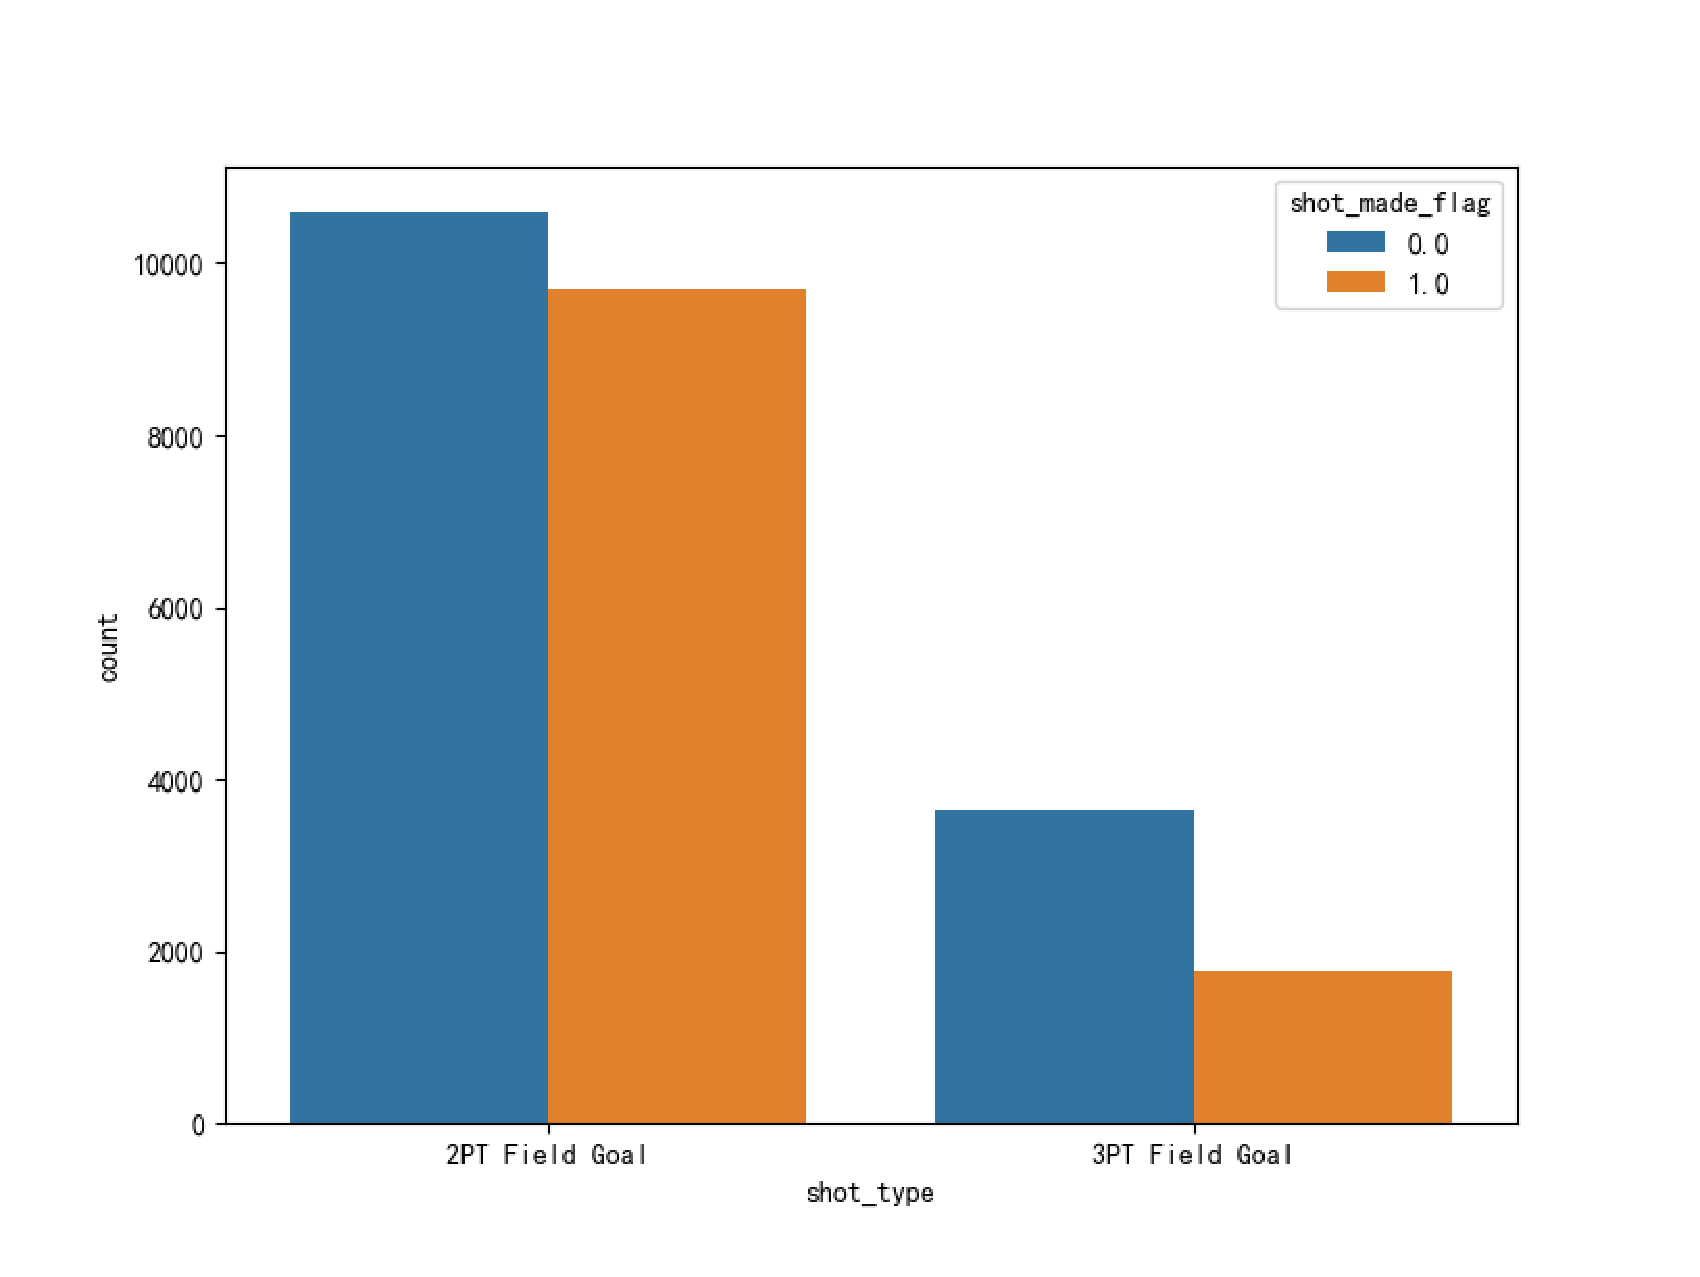
\includegraphics[scale=0.3]{d.eps
	}        %?a??¨º??¨²LaTeX???t?D?D¦Ì??¨¤???¡¤??
	\caption{The hit distribution histogram of two shot types}
	\label{fig1}
\end{figure}

\end{center}
\end{slide}
%%
%%==========================================================================================
\begin{slide}[toc=,bm=]{Data Visualization}
	\begin{center}
		\twotonebox{\rotatebox{90}{Exp}}{\parbox{.96\textwidth}
			{It can be seen that dunk is the highest hit rate, followed by bank shot is about 80\%,
				while jump shot and Tip shot are relatively difficult.
		}}
	\end{center}
	
	\begin{center}
	
		
		\begin{figure}[htbp]
			\centering
			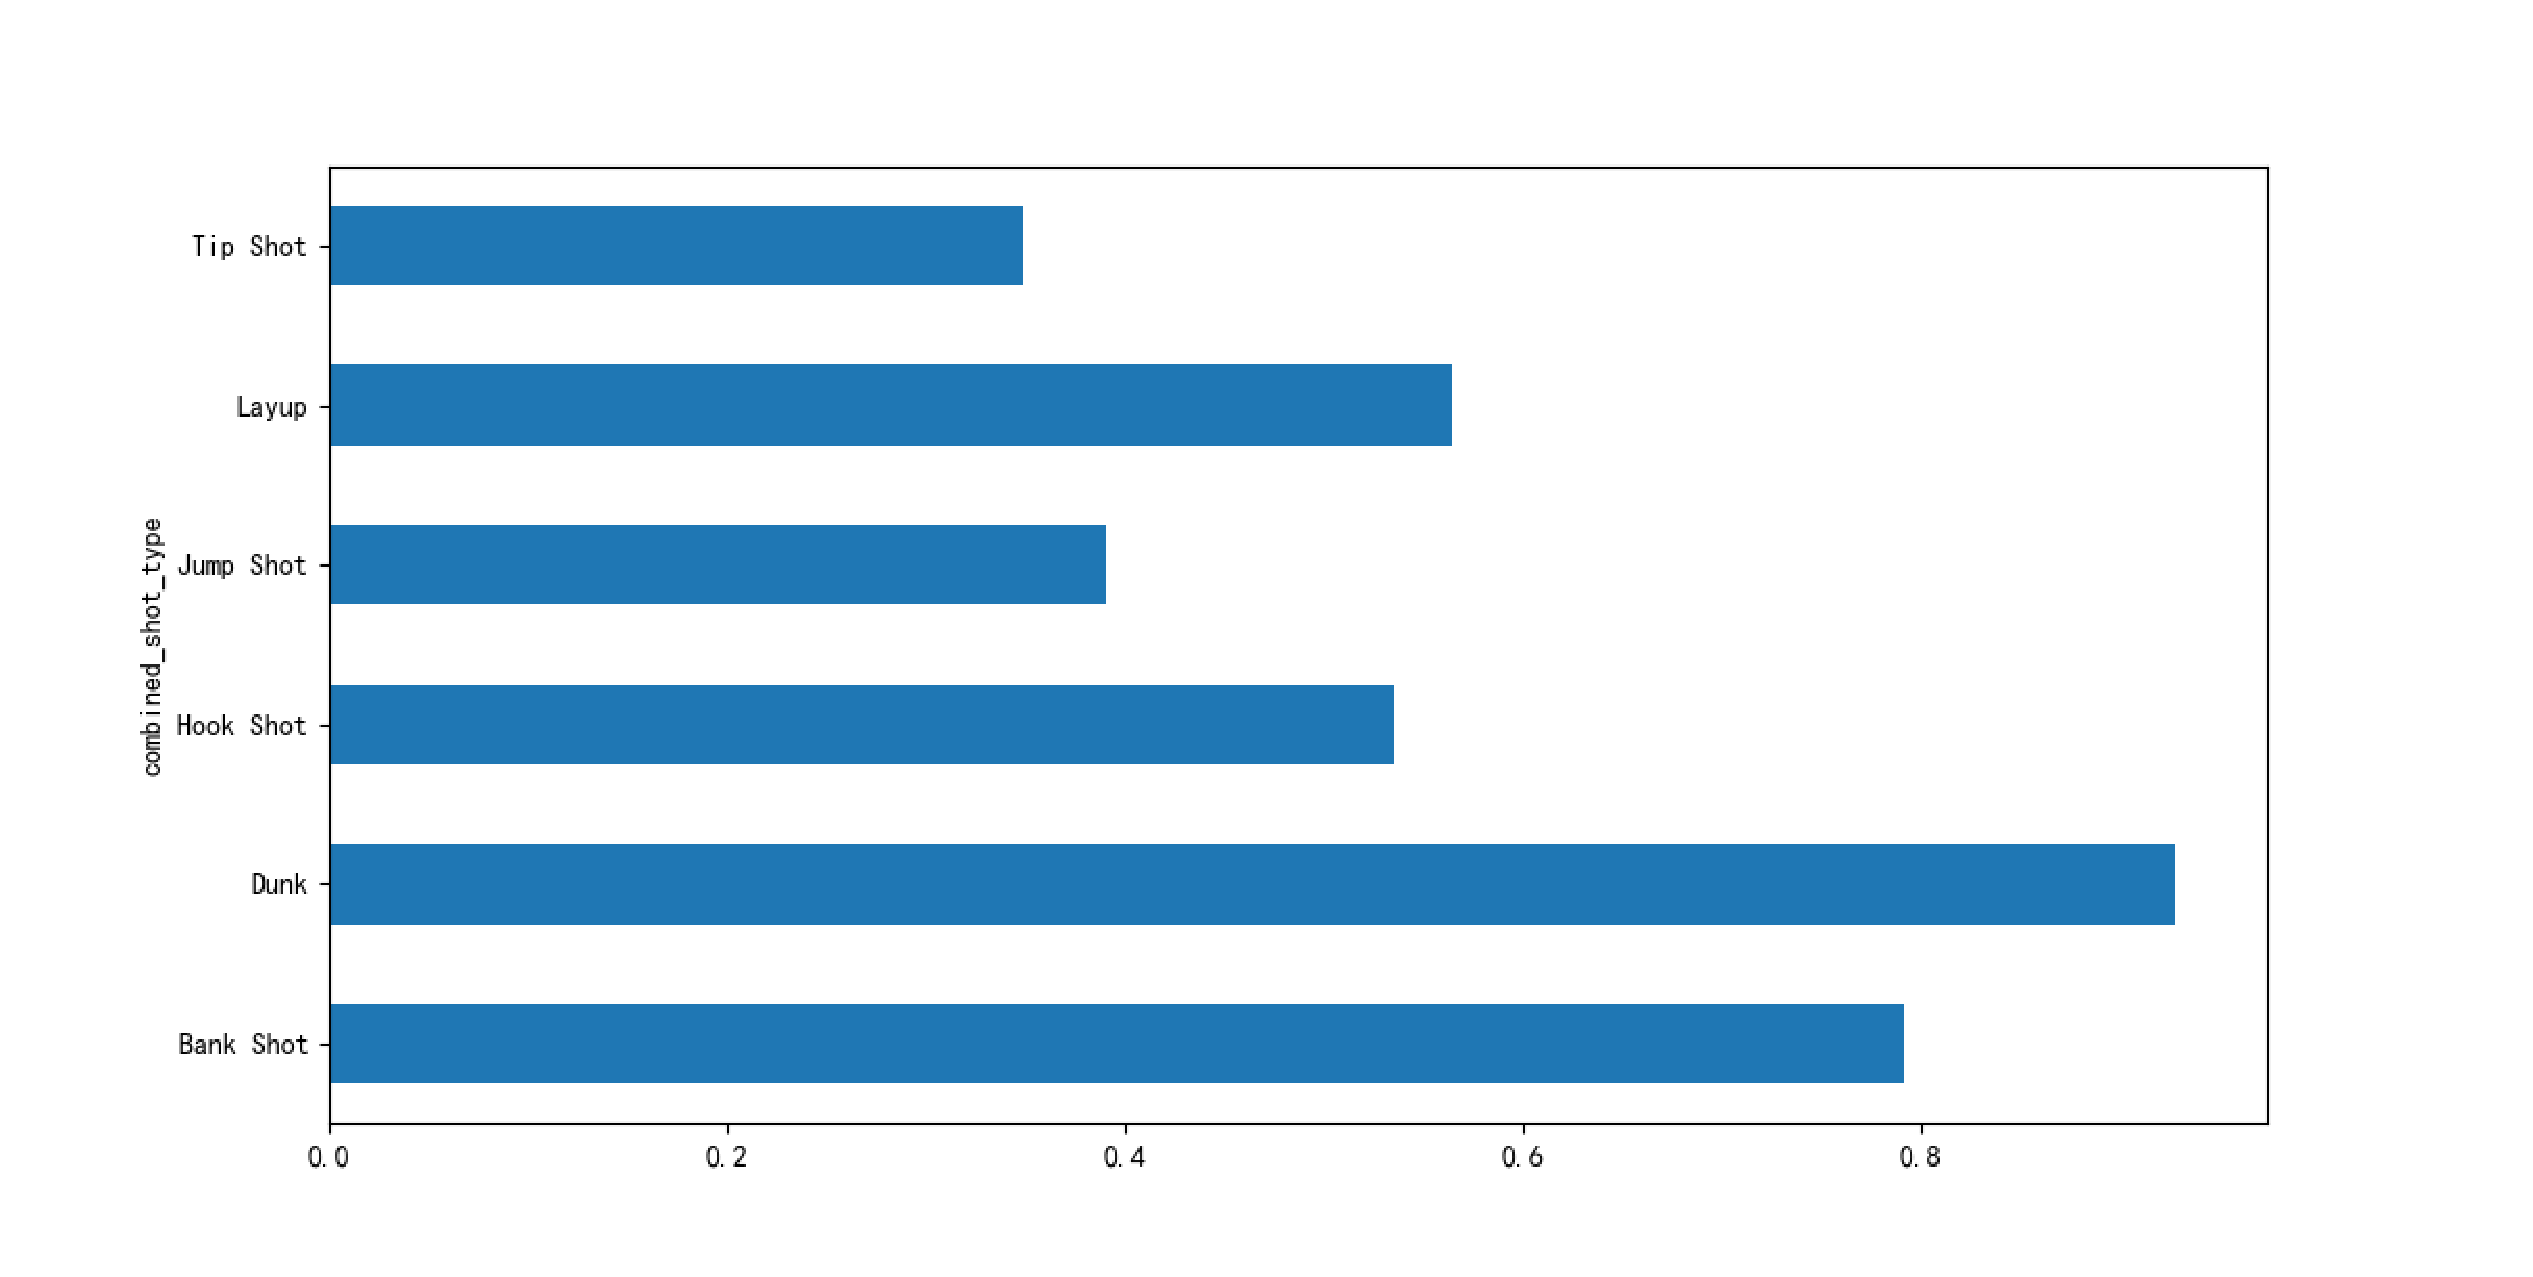
\includegraphics[scale=0.3]{f.eps
			}        %Õâ¸öÊÇÔÚLaTeXÎļþ¼ÐÖеÄÏà¶Ô·¾¶
			\caption{the shot accuracy of various action type}
			\label{fig2}
		\end{figure}
	\end{center}
\end{slide}
%%
%%==========================================================================================

\begin{slide}[toc=,bm=]{Data Visualization}
	\begin{center}
		\twotonebox{\rotatebox{90}{Exp}}{\parbox{.96\textwidth}
			{
				Lets get some understanding about the different zones and the shots made from zones.
		}}
	\end{center}
	
	\begin{figure}[htbp]
		\centering
		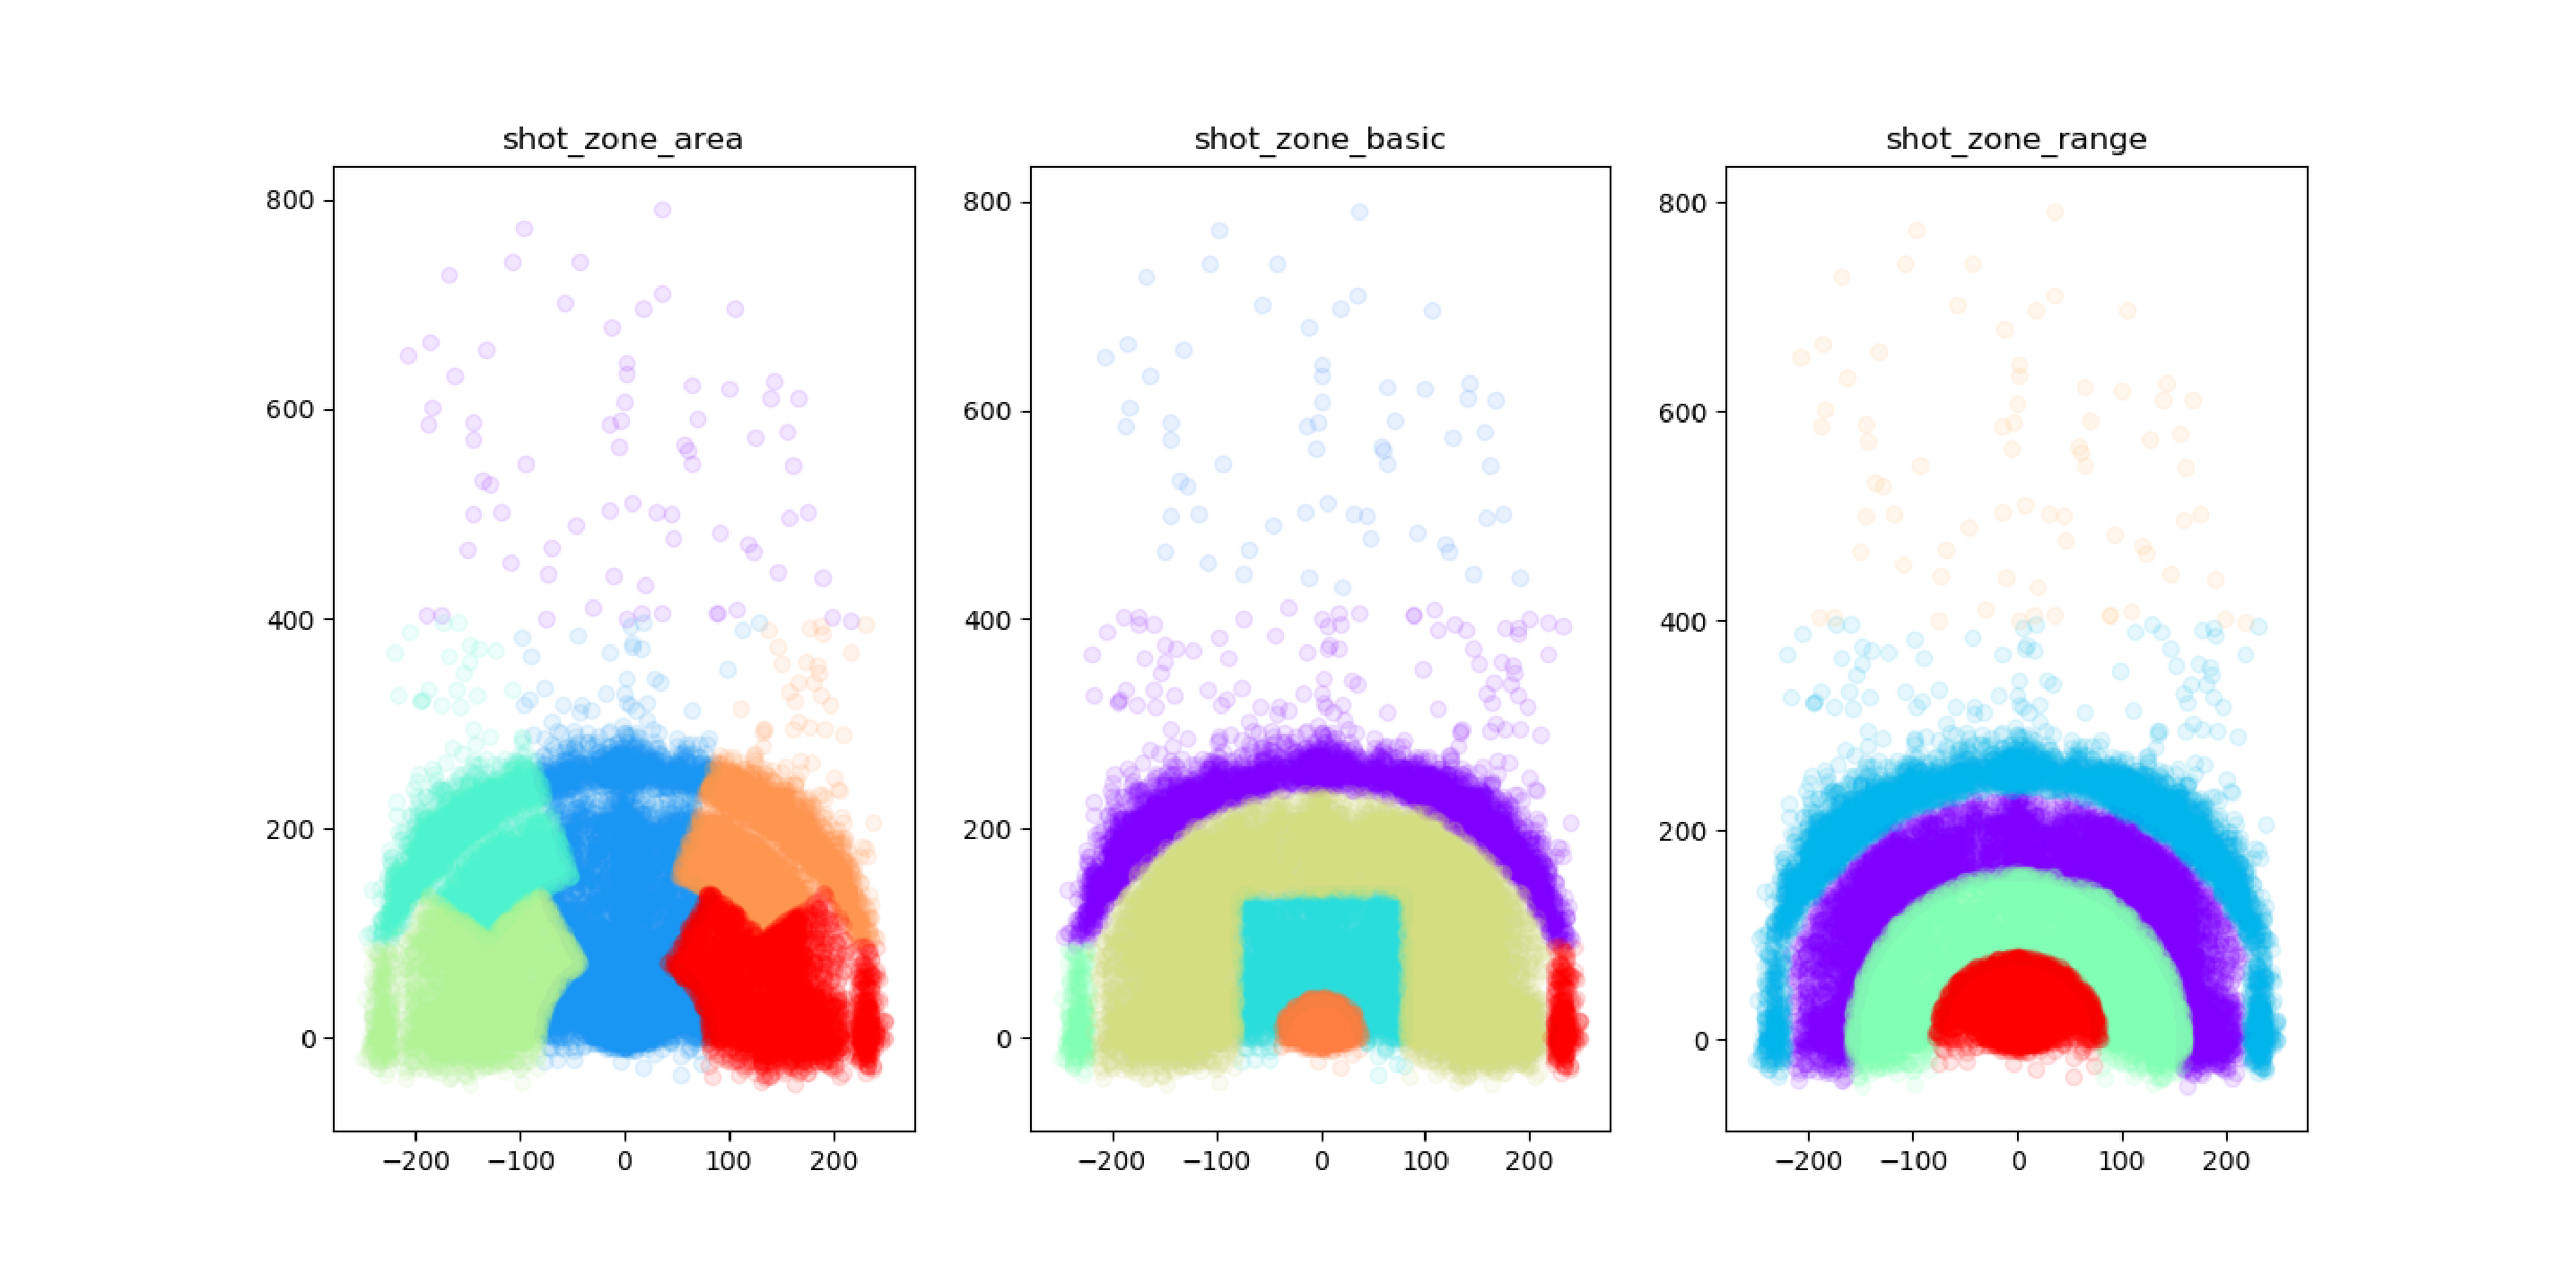
\includegraphics[scale=0.28]{h.eps
		}        %Õâ¸öÊÇÔÚLaTeXÎļþ¼ÐÖеÄÏà¶Ô·¾¶
		\caption{Division of shooting area}
		\label{fig3}
	\end{figure}	

\end{slide}

%%==========================================================================================
%%

\begin{slide}[toc=,bm=]{Data Visualization}
	\begin{center}
		\twotonebox{\rotatebox{90}{Exp}}{\parbox{.96\textwidth}
			{The line chart can not only show the quantity, but also clearly see the increase and decrease of data.
				Lets now see the Kobe's shots positioning with the time and distance.
		}}
	\end{center}
\begin{center}
\begin{figure}[htbp]
	\centering
	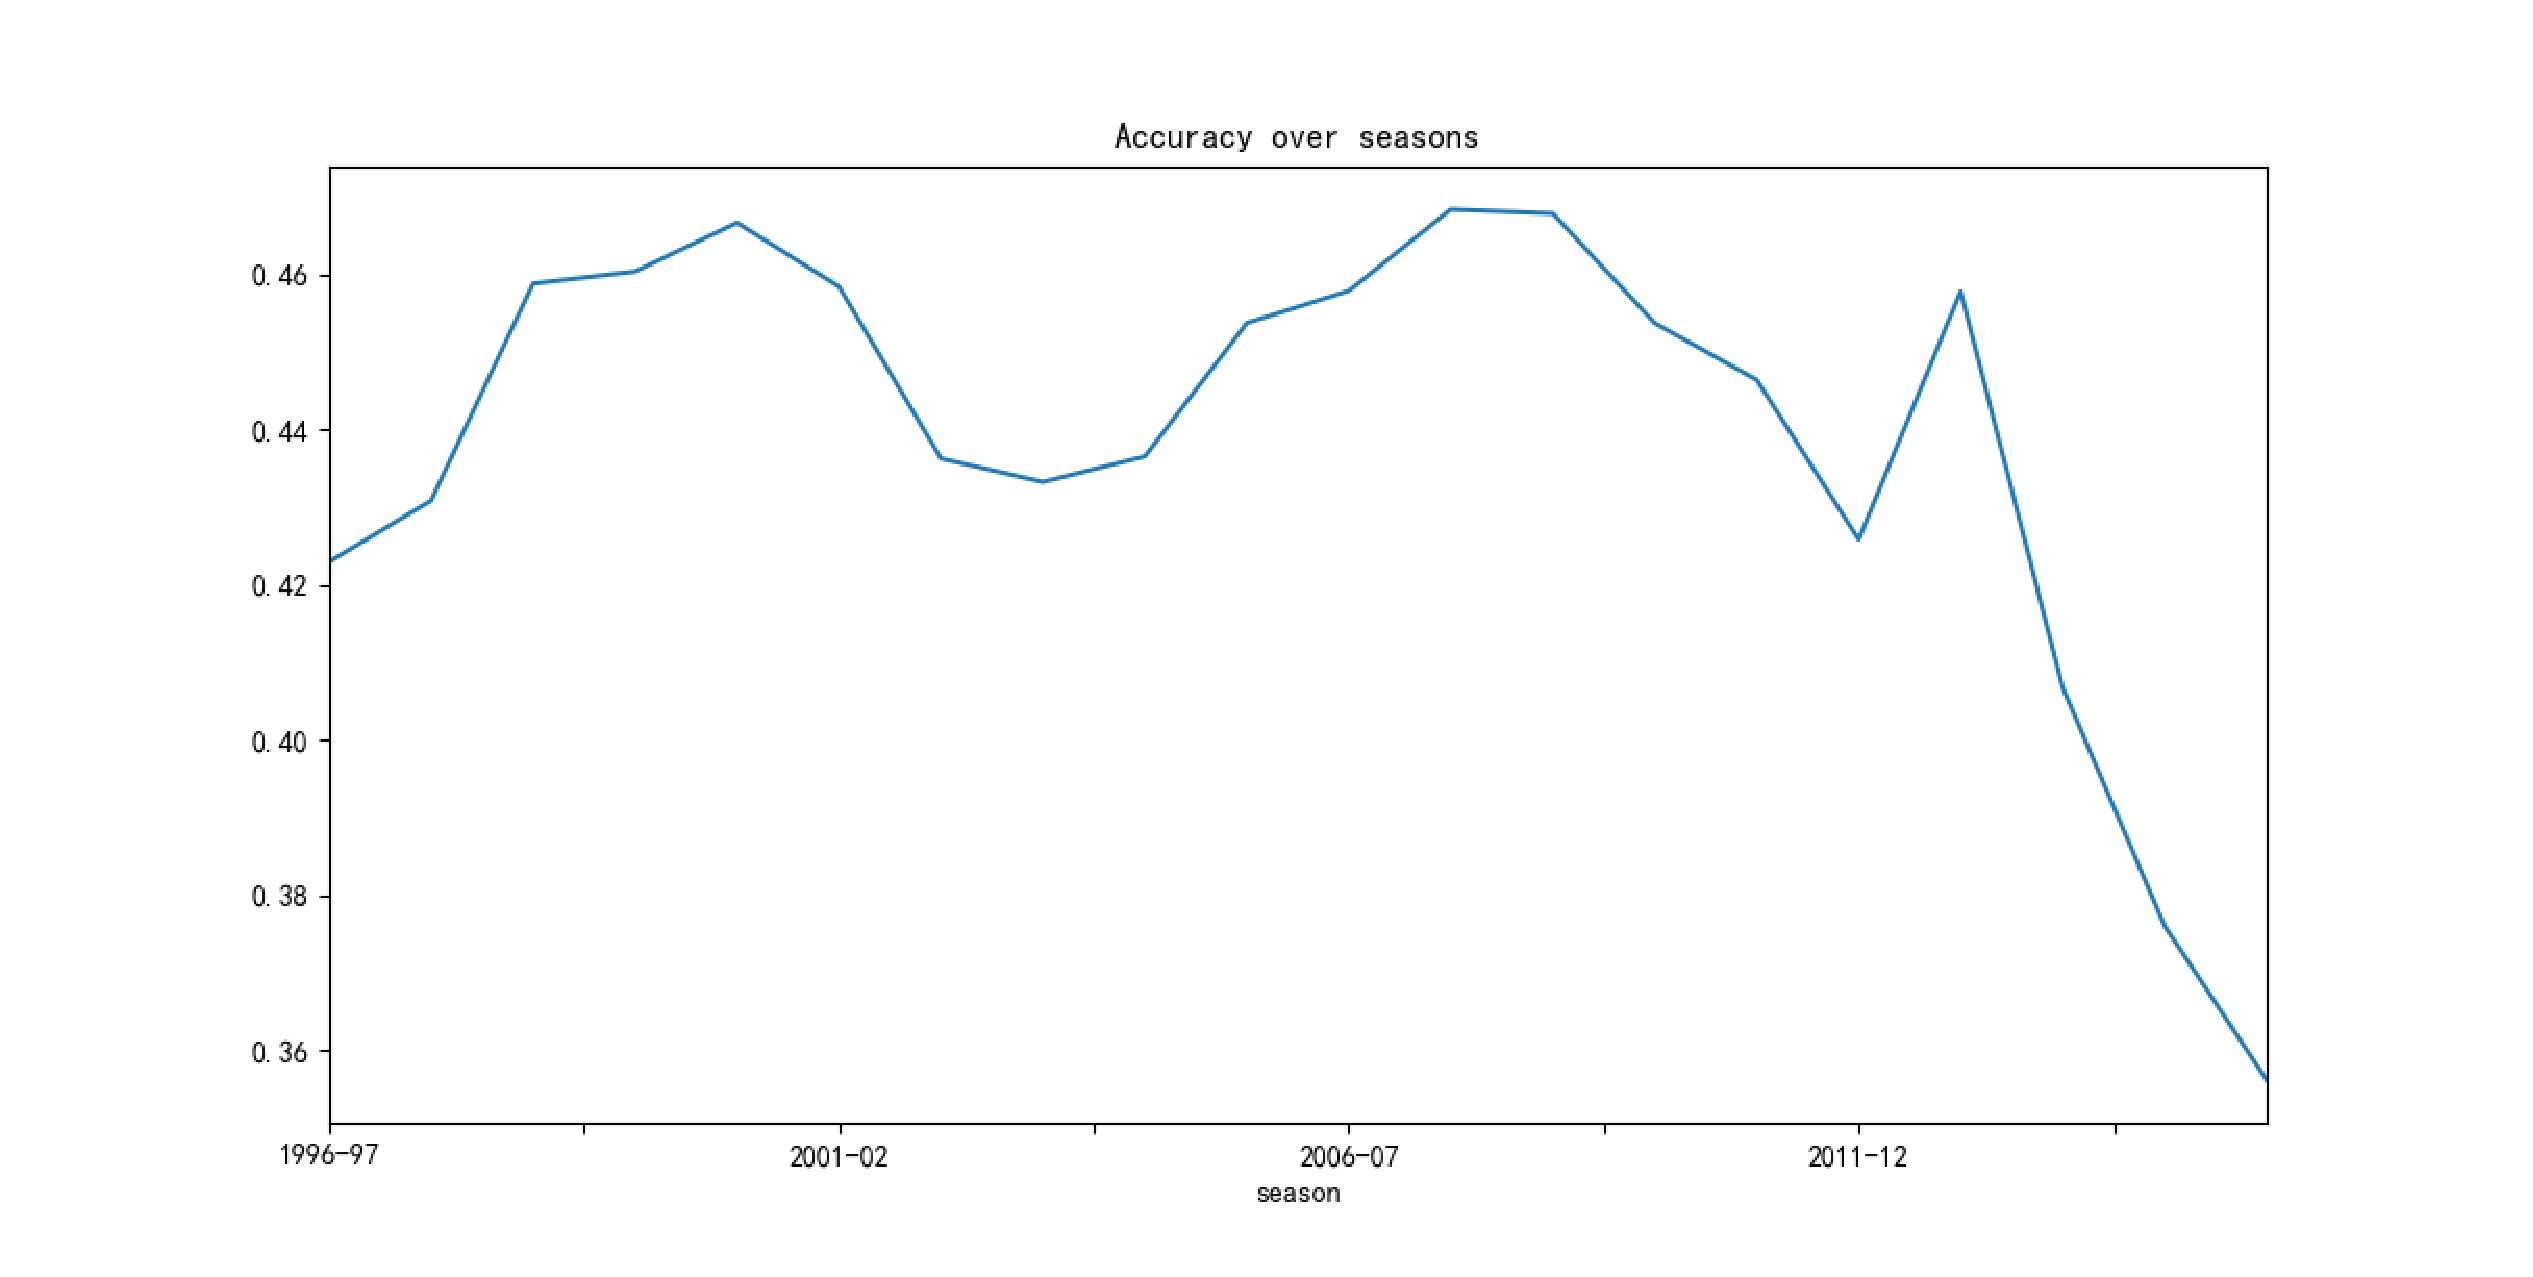
\includegraphics[scale=0.28]{m.eps
	}        %Õâ¸öÊÇÔÚLaTeXÎļþ¼ÐÖеÄÏà¶Ô·¾¶
	\caption{shot accuracy of each seasons}
	\label{fig4}
\end{figure}
\end{center}
\end{slide}
%%==========================================================================================
%%

\begin{slide}[toc=,bm=]{Data Visualization}
	\begin{center}
		\twotonebox{\rotatebox{90}{Exp}}{\parbox{.96\textwidth}
			{The line chart can not only show the quantity, but also clearly see the increase and decrease of data.
				Lets now see the Kobe's shots positioning with the time and distance.
		}}
	\end{center}
	\begin{center}
	\begin{figure}[htbp]
		\centering
		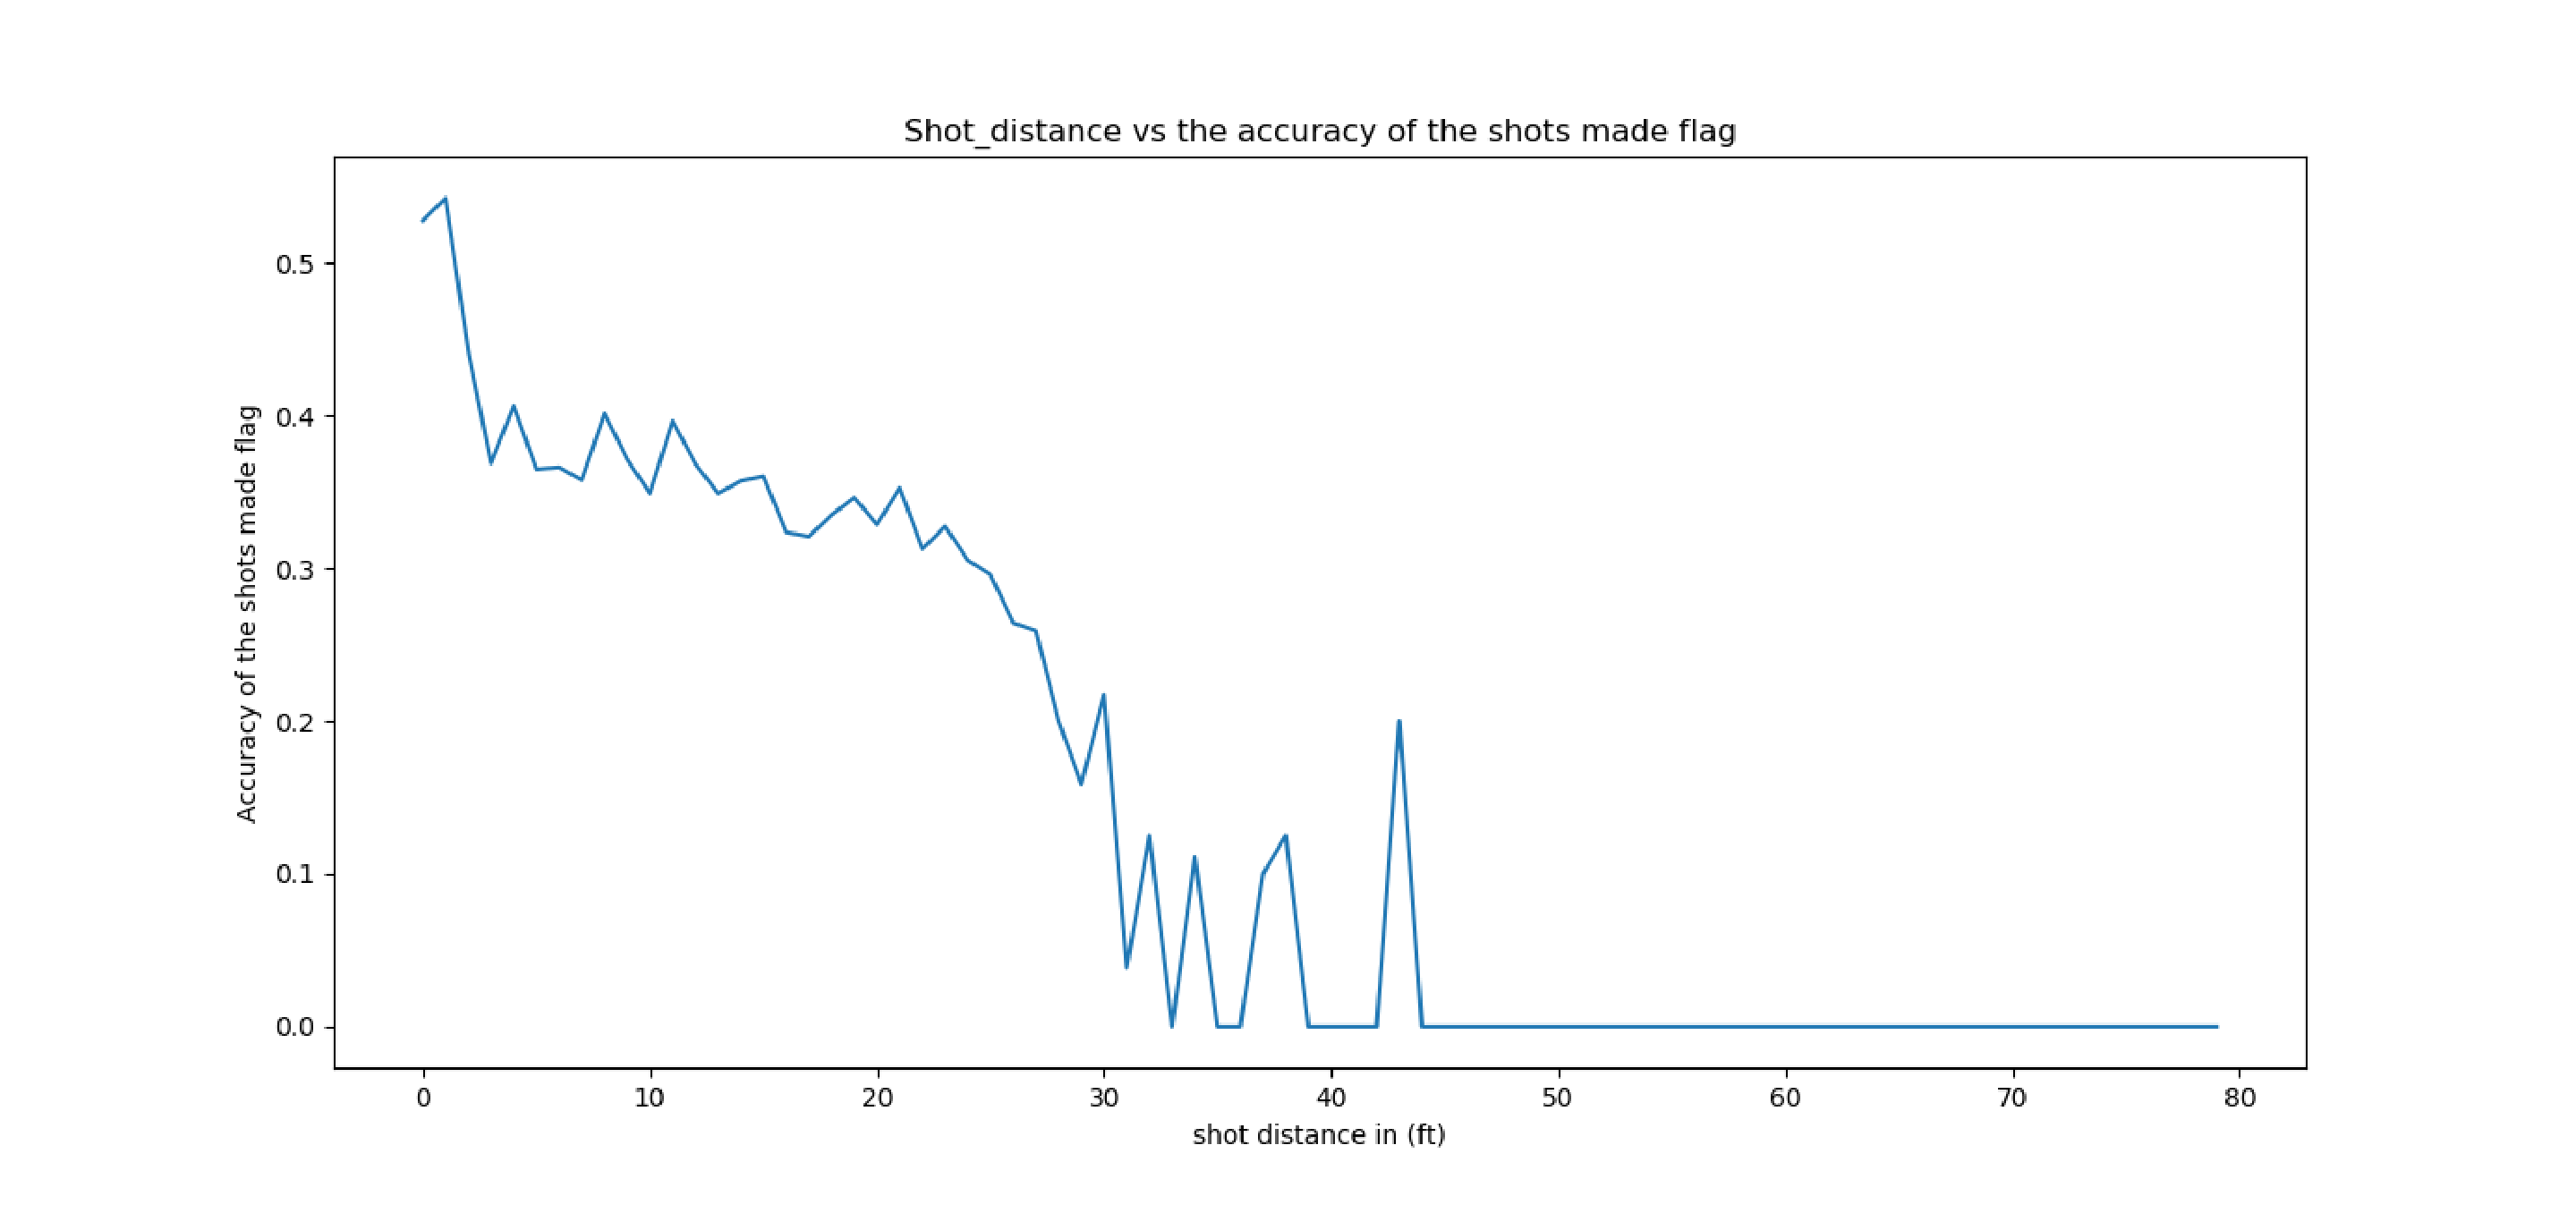
\includegraphics[scale=0.28]{s.eps
		}        %Õâ¸öÊÇÔÚLaTeXÎļþ¼ÐÖеÄÏà¶Ô·¾¶
		\caption{Shot_distance vs the accuracy of the shots made flag}
		\label{fig5}
	\end{figure}
	\end{center}
\end{slide}
%%==========================================================================================
%%
\section{Data Preparation}

\begin{slide}{Data Cleaning}
	\item As it can be seen from 
the picture that, (loc_x ,loc_y) and (lat , lon) represent the same.
So, drop one of those.
	\item Meanwhile,some attributes have no attribution for our model,
Therefore some columns might be dropped.

	\begin{figure}[H]
	\centering
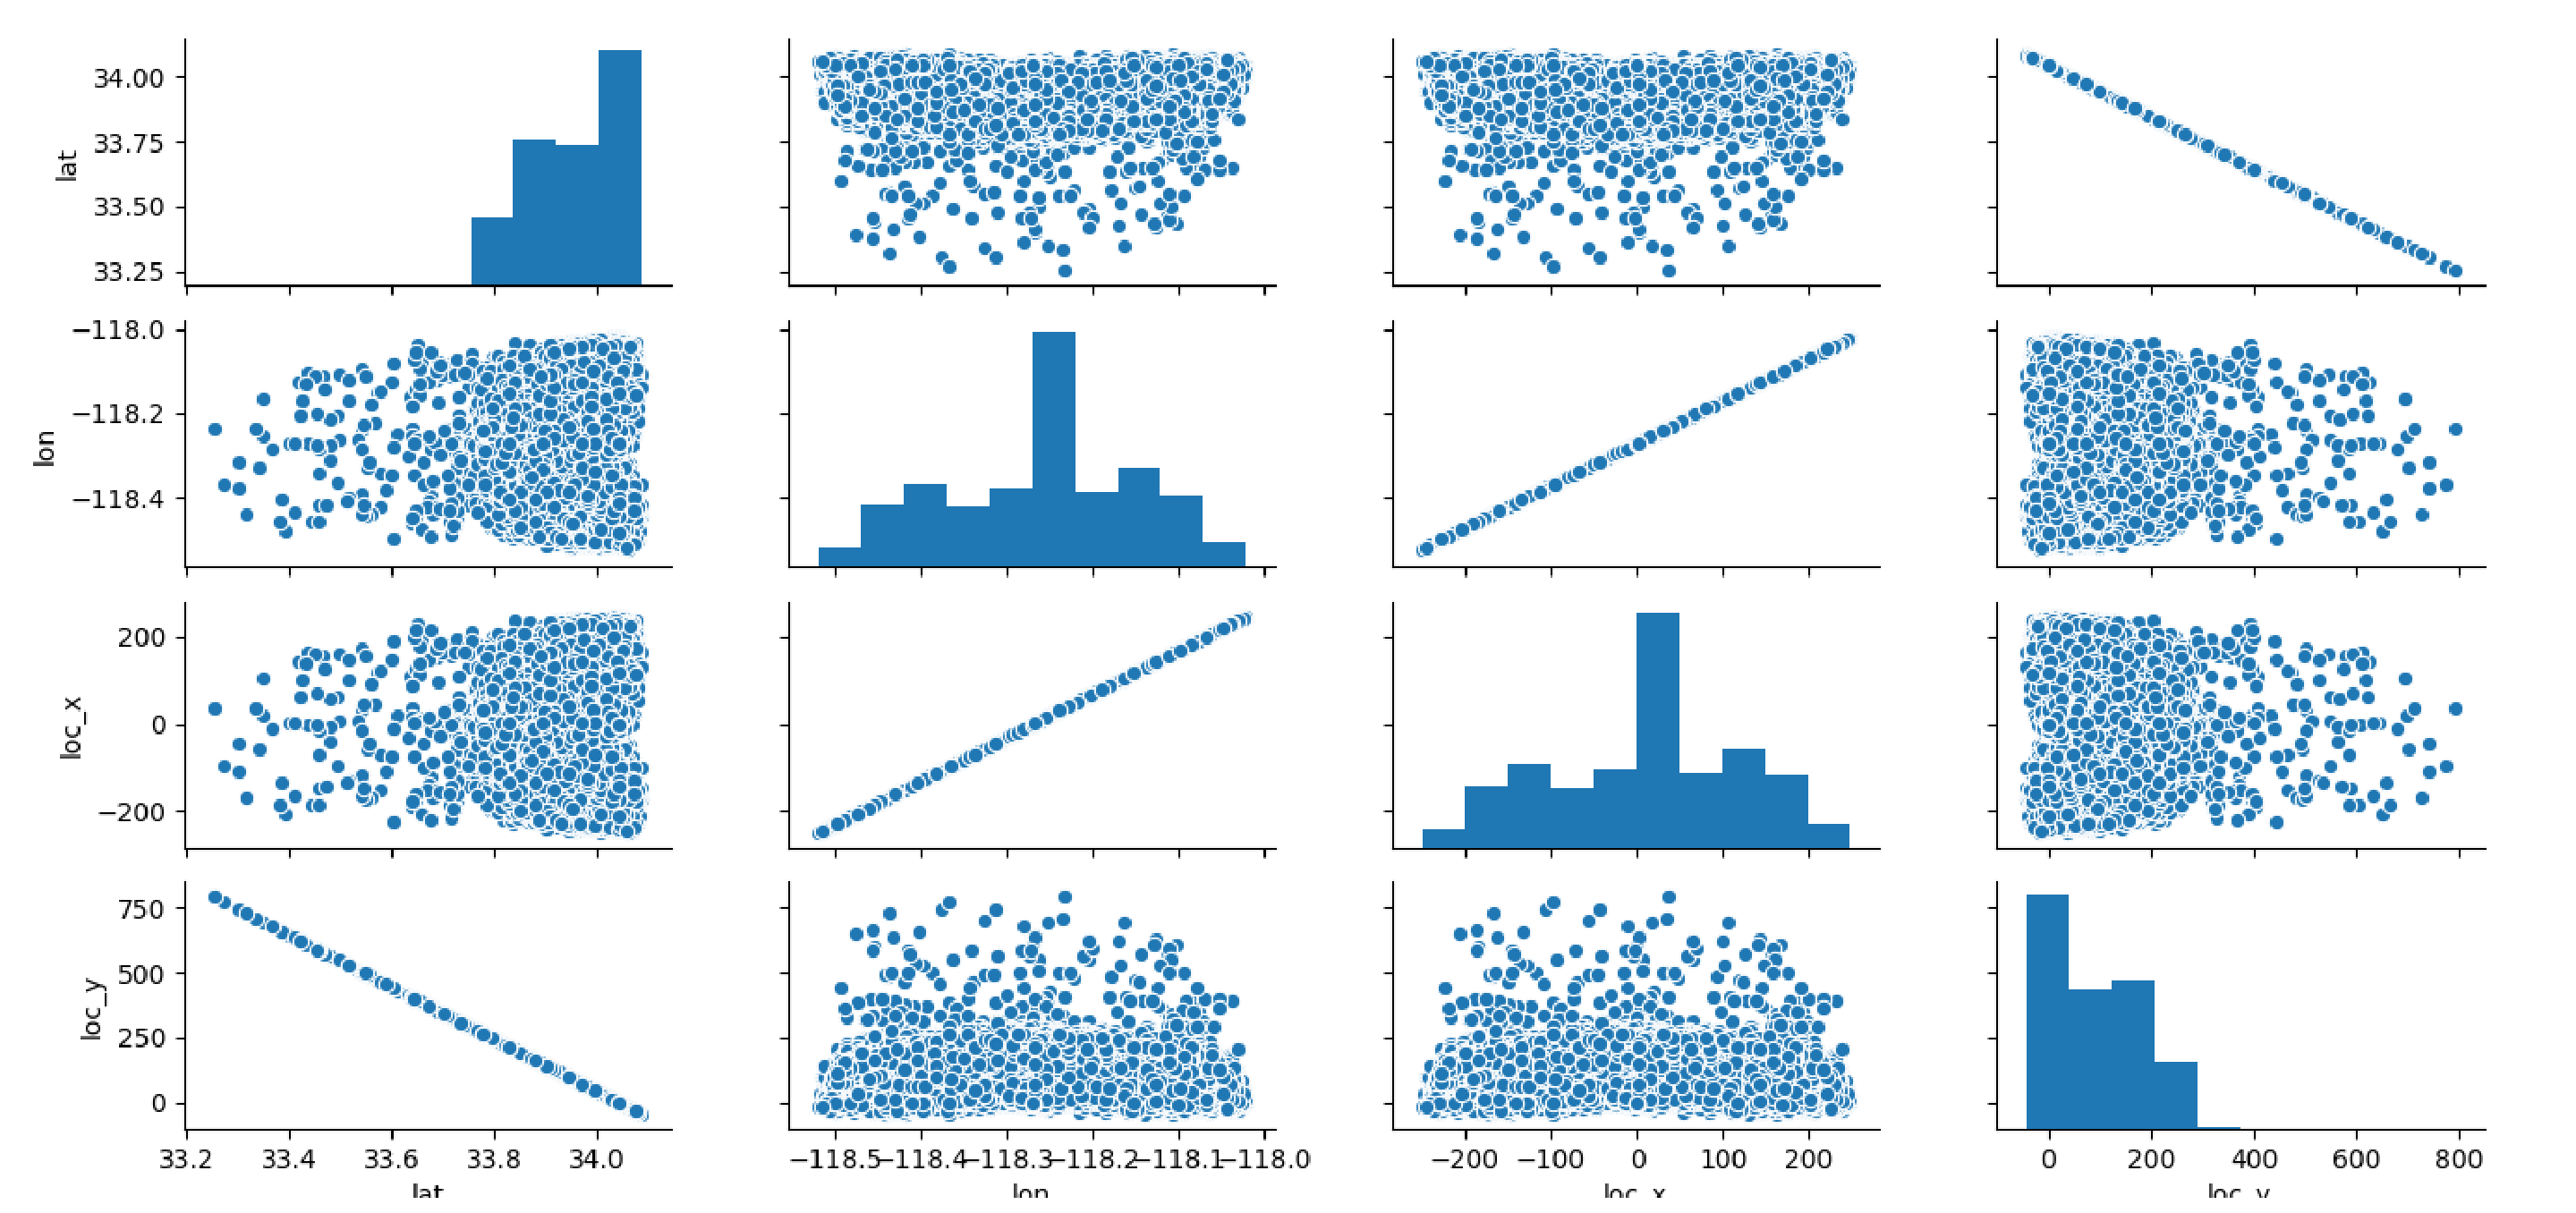
\includegraphics[scale=0.24]{t.eps
}        %Õâ¸öÊÇÔÚLaTeXÎļþ¼ÐÖеÄÏà¶Ô·¾¶
\caption{Pairplot of (loc\_x ,loc\_y) and (lat , lon)}
\label{fig6}
\end{figure}
\end{slide}

\begin{slide}{Data Transformation}

After deleted all the useless columns,we need to \textbf{merge some features},and \textbf{create dummy variables}.\quad
First,Let's convert the minutes and seconds to single column.
\begin{description}
\item total\_seconds = row[seconds\_remaining]+60*row[minutes\_remaining] 
	\newline
After that,we can remove the minutes and the seconds columns.
\end{description}

\item Categorical variables such as \textbf{action_type} , \textbf{combined_shot_type}, \textbf{season}, \textbf{shot_type}, \textbf{shot_zone_range} 
and \textbf{opponent},we can create the dummy variables for further analysis.
\begin{figure}[htbp]
	\centering
	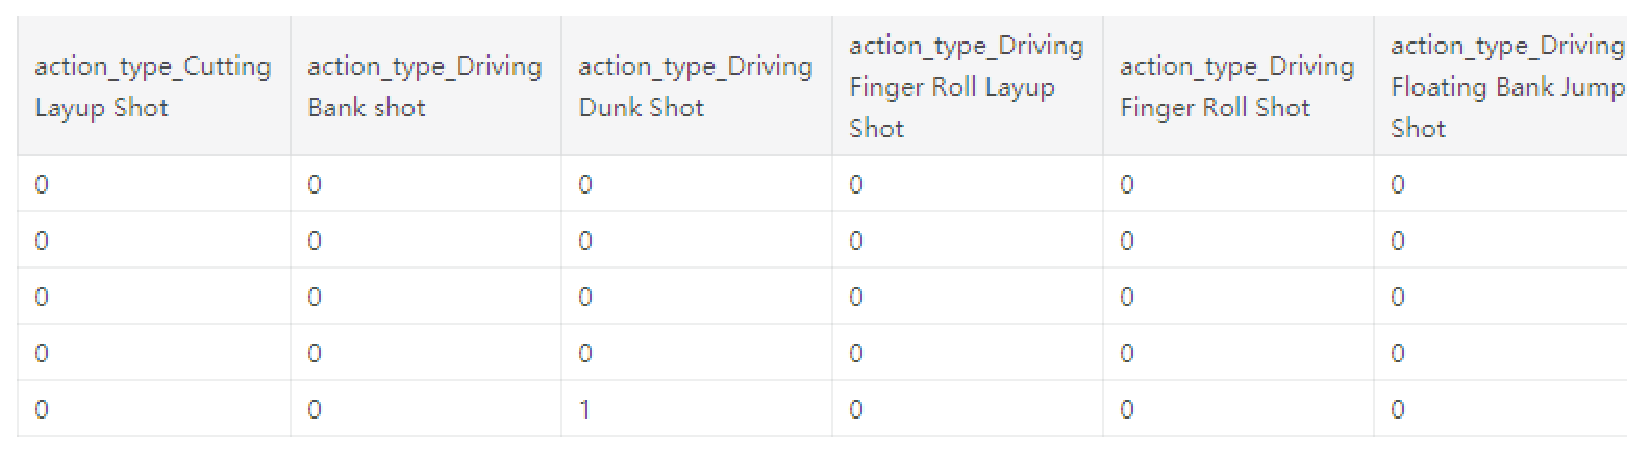
\includegraphics[scale=0.6]{u.eps
	}        %Õâ¸öÊÇÔÚLaTeXÎļþ¼ÐÖеÄÏà¶Ô·¾¶
	\caption{part of the converted dataset}
\end{figure}
\end{slide}
%%=====================================================================


\section{Methods}


%%==========================================================================================
%%
\begin{slide}[toc=,bm=]{Methods}

There are many machine learning algorithms, 
use the machine learning algorithms below
as Ensemble Model’s base models. 
Through Grid Search and
ten-fold cross-validation
to find the optimal parameters.
Then use the ensemble model on
test data.

\begin{center}
	\begin{itemize}
		\item Base Models
		\
		\begin{itemize}
			\item RandomForeset
			\item LogisticRegression	
			\item KNeighbors
		\end{itemize}
	   \item Voting ensemble
	\end{itemize}
\end{center}

\end{slide}

%%==========================================================================================
%%
\begin{slide}{Parameter Adjustment}
	The following are optimal parameters of three models. 
	\begin{itemize}
		\item Best Parameters of Models
	\end{itemize}
	\begin{description}
	\item[RandomForest] 'criterion': 'entropy', 'max\_depth': 5, 
	'max\_features': None, 'n\_estimators': 100
	\item[LogisticRegression] 'C': 1, 'penalty': '11'
	
	\item[KNeighbors] 'algorithm': 'auto', 'leaf\_size': 10, 
	'n\_neighbors': 20, 'p': 5, 'weights': 'uniform'
	
\end{description}
	
\end{slide}

%%
%%==========================================================================================


\section{Make final predictions}


%%==========================================================================================
%%
\begin{slide}{Forecast Results}
The tables below are the accuracy of each model
with the adjusted optimal parameter.
\begin{itemize}
	\item Metrics Classification Report of Ensemble Model in original and new train data
\end{itemize}
\begin{center}
\item {Accuracy of three Models}
	\begin{tabular}{cccc}
	%\bottomrule
	\toprule
	& RF  & LR  & KNN \\
	\midrule
	Best Score & 0.637509727626  & 0.68186770428  & 0.568404669261 \\
	\bottomrule
\end{tabular}
\end{center}
\begin{description}
	\item It has shown that logistic regression runs better than others.In the final model, the weights of LR is larger.
\end{description}
\begin{description}
	\item Then,use the ensemble model make the final prediction.	The final ensemble model's prediction accuracy is \textbf{0.738894059077}.
		\newline
	Finally, generate the forecast result and save them in the csv file.
\end{description}




\end{slide}


%%
%%==========================================================================================


%%
%%==========================================================================================


\section{Conclusion}

%%==========================================================================================
%%
\begin{slide}[toc=,bm=]{Conclusion}
\begin{description}
	\item[Exploratory Data Analysis] It is an 
	exploratory analysis of the data to 
	provide the necessary conclusions 
	for data processing and modeling.
	\item[Data Preprocessing] This step contains
	dealing with missing data and outliers,
	changing categorical variable 
	into one-hot code and so on.
	\item[Feature Engineering] It's the 
	most important thing.
	Create as more as poosible features,
	then select the most useful features.
	\item[Model Training] The models have 
	many parameters,
	and can use Grid Search to find 
	the optimal paratemers.	
\end{description}



\end{slide}
%%
%%==========================================================================================


%%==========================================================================================
%

\section{Thanks for attending and welcome for questions}
%%
%%==========================================================================================


%%==========================================================================================
% TODO: Contact Page

\end{document}

\endinput
